\subsection{Toolsuite Used for Implementation}
%The algorithms in this paper are implemented in the Safety Annex for the Architecture Analysis and Design Language (AADL) and require the Assume-Guarantee Reasoning Environment (AGREE)~\cite{NFM2012:CoGaMiWhLaLu} to annotate the AADL model in order to perform verification using the back-end model checker \jkind~\cite{2017arXiv171201222G}. 

\textbf{Architecture Analysis and Design Language}
We are using the Architectural Analysis and Design Language (AADL) to construct system architecture models of performance-critical, embedded, real-time systems~\cite{AADL_Standard}. %An AADL model describes a system in terms of a hierarchy of components and their interconnections, where each component can either represent a logical entity (e.g., application software functions, data) or a physical entity (e.g., buses, processors). 
Language annexes to AADL provide a rich set of modeling elements for various system design and analysis needs, and the language definition is sufficiently rigorous to support formal analysis tools that allow for early fault detection. 
\begin{comment}
Figure~\ref{fig:tempSensor} shows a temperature sensor component defined in AADL. It has a single input (\texttt{Env\_Temp}) and a single output (\texttt{High\_Temp\_Indicator}).  

\begin{figure*}[h!]
	\vspace{-2em}
	\begin{center}
		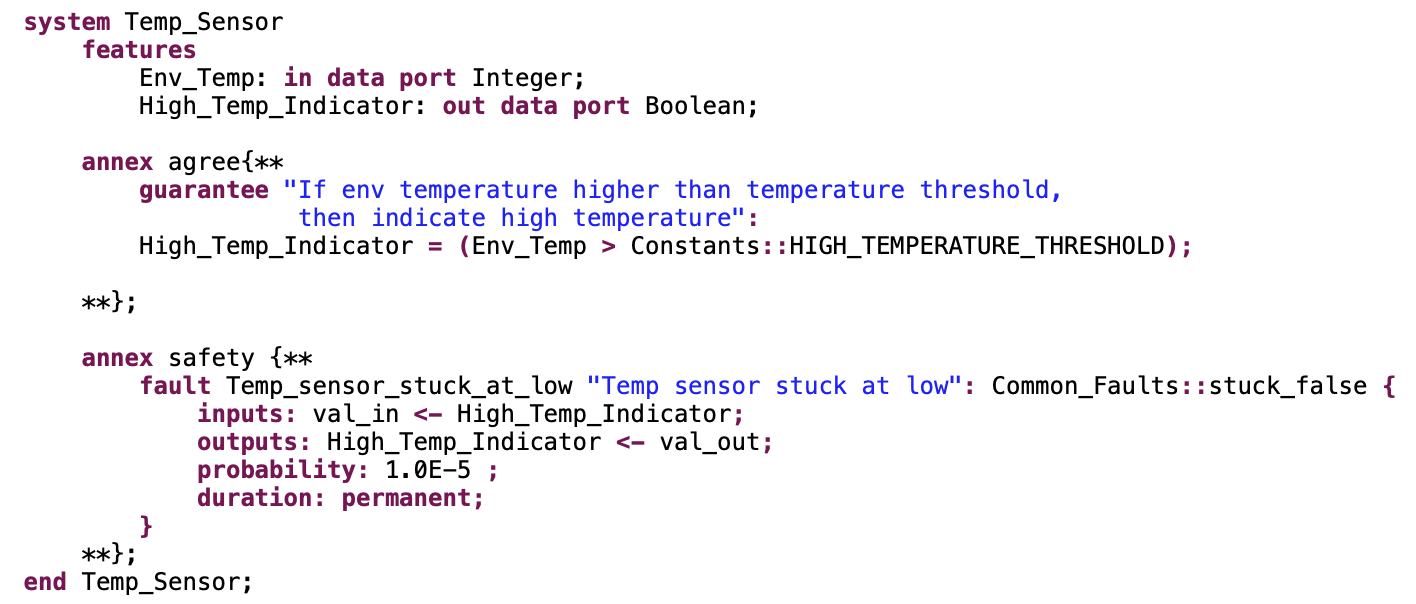
\includegraphics[width=0.9\textwidth]{images/tempSensoraadlannex.png}
	\end{center}
	\vspace{-2em}
	\caption{Temperature sensor in AADL with AGREE and safety annexes}
	\label{fig:tempSensor}
	\vspace{-2em}
\end{figure*}
\end{comment}

%\textbf{Compositional Analysis} 
%One way to structure compositional verification is hierarchically: layers of the system architecture are analyzed independently and their composition demonstrates a system property of interest. Compositional verification partitions the formal analysis of a system architecture into verification tasks that correspond into the decomposition of the architecture~\cite{clarke1989compositional}.  A proof consists of demonstrating that the system property is provable given the contracts of its direct subcomponents and the system assumptions~\cite{cofer2012compositional,clarke1989compositional}. When compared to monolithic analysis (i.e., analysis of the flattened model composed of all components), the compositional approach allows the analysis to scale to much larger systems~\cite{NFM2012:CoGaMiWhLaLu,heckel1998compositional,cofer2012compositional}.

\textbf{Assume Guarantee Reasoning Environment}
The Assume Guarantee Reasoning Environment (AGREE) is a tool for formal analysis of behaviors in AADL models and supports compositional verification~\cite{NFM2012:CoGaMiWhLaLu}.  It is implemented as an AADL annex and is used to annotate AADL components with formal behavioral contracts. Each component's contracts includes assumptions and guarantees about the component's inputs and outputs respectively. AGREE translates an AADL model and the behavioral contracts into Lustre~\cite{Halbwachs91:IEEE} and then queries the \jkind model checker to conduct the back-end analysis~\cite{2017arXiv171201222G}. %Figure~\ref{fig:tempSensor} shows the guarantee defined in the temperature sensor written in the AGREE annex.

%\textbf{JKind}
%JKind is an open-source industrial infinite-state inductive model checker for safety properties~\cite{2017arXiv171201222G}. Models and properties in JKind are specified in Lustre~\cite{Halbwachs91:IEEE}, a synchronous dataflow language, using the theories of linear real and integer arithmetic. JKind uses SMT-solvers to prove and falsify multiple properties in parallel.

\textbf{Safety Annex for AADL}
The Safety Annex for AADL provides the ability to reason about faults and faulty component behaviors in AADL models~\cite{Stewart17:IMBSA,stewart2020safety}. In the safety annex approach, AGREE is used to define the nominal behavior of system components, faults are introduced into the nominal model, and the JKind model checker is used to analyze the behavior of the system in the presence of faults. %Faults describe deviations from the nominal behavior and are attached to the outputs of components in the system. An example of a safety annex fault definition on the temperature sensor is shown in Figure~\ref{fig:tempSensor}. The fault is associated with the \texttt{High\_Temp\_Indicator} output and has a probability of occurrence of $1.0 \times 10^{-5}$. The behavior of the output when the fault is active is to report low temperature. 